\section{实验材料及方法}
本文是将商用AZ31B镁合金板材和1060纯铝板材制成铝-镁-铝夹层,进行不同道次及道次压下率复合轧制实验,并对轧制所得板材进行显微组织观察及力学性能分析研究。本章介绍了实验所采用的材料、样品制备方式及实验方法。\par
\subsection{实验流程图}
图\ref{fig:liuchengtu}所示为实验流程图。对试样轧制复合后,主要利用相关仪器设备测试分析微观组织和力学性能。\par

%顶部对齐,将空白集中到页面底部
\raggedbottom

\begin{figure}[H]
	\vspace{-0.5em}
	\centering
	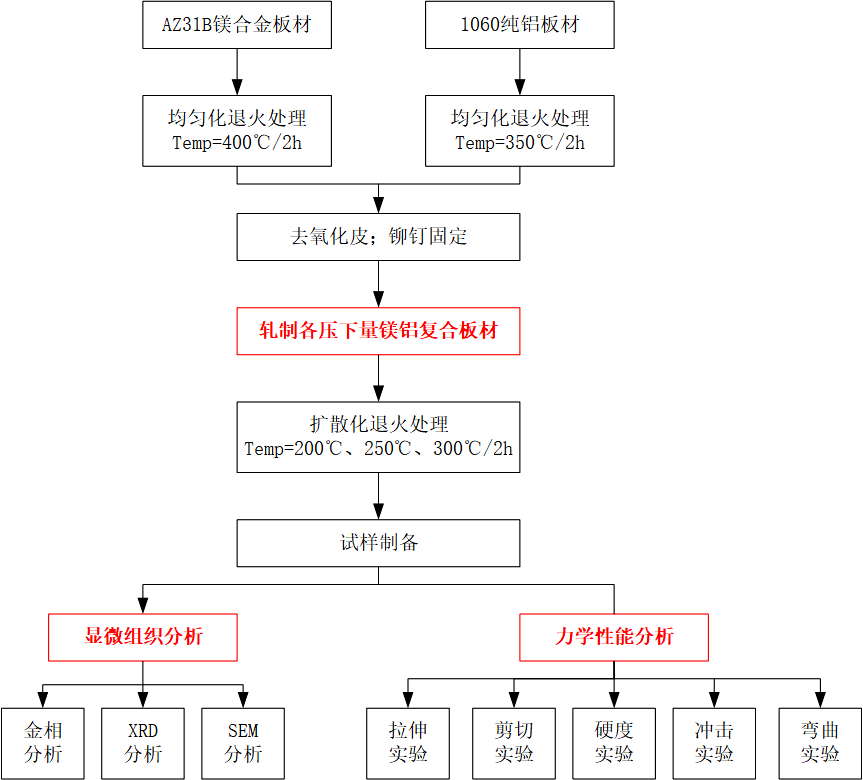
\includegraphics[width=0.8\textwidth]{images/liuchengtu.png}
	\caption{情感倾向分析流程}
	\label{fig:liuchengtu}
	\vspace{-1.5em}
\end{figure}
\subsection{实验材料}
实验所采用的原始材料为商用AZ31B镁合金铸轧板材和1060铝板材。合金原材料采用连续铸轧工艺生产,生产工序经过配料/熔炼/静置/放料/连续铸轧等流程,由于原材料板材较大,采用剪板机进行切割取样。\par
\subsection{样品制备}
\subsubsection{镁铝夹层的制备}
轧制前准备好8块镁合金板材和16块铝合金板材样品,镁板和铝板厚度均为2mm,将镁板放入加热炉进行400℃均匀化退火处理2小时,铝板放入加热炉进行350℃均匀化退火处理2小时。\par


\subsubsection{金相试样制备}
因为轧制获得的镁铝复合板材存在边缘裂纹等缺陷,需要利用线切割机床进行切割取样,其中金相观察部分中,对未退火及各退火温度(200℃、250℃、300℃)的轧制后板材各取3个试样,切割成矩形小块,分别用于观察表面金相组织、镁铝界面相组织。\par
\subsubsection{XRD试样制备}
制备XRD试样时,先用600$\#$、1000$\#$、2000$\#$砂纸将表面打磨平整、去除表面氧化皮并清洁干净,随后取一张干净的滤纸,将样品放置在铝合金框架中间,用橡皮泥固定,使待观察的试样表面与铝合金框架平齐,处于同一平面上。\par
\subsection{实验方法}
\subsubsection{金相观察}
在金相观察前,先用普通光学显微镜观察腐蚀效果,如能观察到清晰的晶界且没有明显缺陷,则改用金相显微镜观察记录,观察时进行图像采集并添加标尺。\par
\subsubsection{扫描电镜(SEM)分析}
扫描电镜(SEM)的主要原理是利用聚焦电子束照射在试样表面所激发出来的一系列物理信号所形成的图像。入射电子束和样品表面作用后会产生很大电子信号,譬如吸收电子、背散射电子、透射电子、二次电子和特征 X 射线。 \par

\clearpage